\documentclass{ximera}

\begin{document}
	\author{Stitz-Zeager}
	\xmtitle{TITLE}


\mfpicnumber{1}

\opengraphsfile{RadianMeasure}

\setcounter{footnote}{0}

\label{RadianMeasure}

In Section \ref{AppAngles},  we review the concept of (oriented) angles and degree measure.  While  degrees are the unit of choice for many applications of trigonometry, we introduce here the concept of the \index{angle ! radian measure}\index{radian measure}\textbf{radian measure} of an angle.  As we will see, this concept naturally ties angles to real numbers.  While the concept may seem foreign at first, we assure the reader that the utility of radian measure in modeling real-world phenomena is well worth the effort.  We begin our development with a definition from Geometry.


\smallskip

\colorbox{ResultColor}{\bbm

\begin{defn} \label{pidefn} \index{pi, $\pi$} The real number $\pi$ is defined to be the ratio of a circle's circumference to its diameter.  In symbols, given a circle of circumference $C$ and diameter $d$, 

\[ \pi = \dfrac{C}{d} \]

\end{defn}

\ebm}

\smallskip

While Definition \ref{pidefn} is quite possibly the `standard' definition of $\pi$, the authors would be remiss if we didn't mention that buried in this definition is actually a theorem.  As the reader is probably aware, the number $\pi$ is a mathematical constant - that is, it doesn't matter \textit{which} circle is selected, the ratio of its circumference to its diameter will have the same value as any other circle.  While this is indeed true, it is far from obvious and leads to a  counterintuitive scenario which is explored in the Exercises.   Since the diameter of a circle is twice its radius, we can quickly rearrange the equation in Definition \ref{pidefn} to get a formula more useful for our purposes, namely: $2 \pi = \frac{C}{r}$.  Hence, for any circle,  the ratio of its circumference to its radius is $2\pi$.

\smallskip

Suppose we take a \textit{portion} of the circle as depicted below, and we compare some arc measuring $s$ units in length to the radius.  Let $\theta$ be the \textbf{central angle}\index{angle ! central angle}\index{central angle} subtended by this arc, that is, an angle whose vertex is the center of the circle and whose determining rays pass through the endpoints of the arc.  Using proportionality (similarity) arguments, it stands to reason that the ratio $\frac{s}{r}$ should also be a constant among all circles.  It is this ratio, $\frac{s}{r}$, which defines the \textbf{radian measure} of an angle.

\begin{center}


\begin{mfpic}[20]{-5}{5}{-5}{5}
\drawcolor[gray]{0.7}
\circle{(0,0),3}
\drawcolor{black}
\arrow \reverse \arrow \parafcn{5, 115, 5}{1.5*dir(t)}
\tlabel[cc](0.75, 1.75){$\theta$}
\penwd{1.25pt}
\arrow \reverse \arrow \polyline{(5, 0), (0,0), (-2.5, 4.3301)}
\penwd{1.5pt}
\parafcn{0,120,5}{3*dir(t)}
\tlabel[cc](1.75,3.1){$s$}
\tlabel[cc](1.5,-0.5){$r$}
\tlabel[cc](-1.5,1){$r$}
\point[4pt]{(0,0)}
\end{mfpic} 


The radian measure of $\theta$ is $\dfrac{s}{r}$. 

\end{center}


To get a better feel for radian measure, we note that an angle with radian measure $1$ means the corresponding arc length $s$ equals the radius of the circle $r$, that is,  $s = r$.  When the radian measure is $2$, we have $s = 2r$; when the radian measure is $3$, $s = 3r$, and so forth.  Thus the radian measure of an angle $\theta$ tells us how many `radius lengths' we need to sweep out along the circle to subtend the angle $\theta$.


\begin{center}
\begin{tabular}{cc}

\begin{mfpic}[20]{-5}{5}{-5}{5}
\point[4pt]{(0,0)}
\drawcolor[gray]{0.7}
\circle{(0,0),3}
\drawcolor{black}
\arrow \reverse \arrow \parafcn{5, 52, 5}{1.5*dir(t)}
\tlabel[cc](1.755, 0.9588){$\alpha$}
\penwd{1.25pt}
\arrow \reverse \arrow \polyline{(5, 0), (0,0), (2.70, 4.21)}
\penwd{1.5pt}
\parafcn{0,57.30,5}{3*dir(t)}
\point[4pt]{(3,0), (1.62, 2.52)}
\tlabel[cc](3.12,1.71){$r$}
\tlabel[cc](1.5,-0.5){$r$}
\tlabel[cc](0.5,1.5){$r$}
\end{mfpic} 

\hspace{.5in}
& 

\begin{mfpic}[20]{-5}{5}{-5}{5}
\point[4pt]{(0,0)}
\drawcolor[gray]{0.7}
\circle{(0,0),3}
\drawcolor{black}
\arrow \reverse \arrow \parafcn{5, 225, 5}{1.5*dir(t)}
\tlabel[cc](-0.83, 1.82){$\beta$}
\penwd{1.25pt}
\arrow \reverse \arrow \polyline{(5, 0), (0,0), (-3.268, -3.784)}
\penwd{1.5pt}
\parafcn{0,229.18,5}{3*dir(t)}
\point[4pt]{(3,0), (1.62, 2.52), (-1.25, 2.73), (-2.97, 0.42), (-1.96, -2.27)}
\tlabel[cc](3.12,1.71){$r$}
\tlabel[cc](0.25,3.55){$r$}
\tlabel[cc](-2.84,2.12){$r$}
\tlabel[cc](-3.74,-1.24){$r$}
\tlabel[cc](1.5,-0.5){$r$}
\tlabel[cc](-.5,-1.23){$r$}
\end{mfpic}  \\


$\alpha$ has radian measure $1$ 
\hspace{.5in}

& $\beta$ has radian measure $4$

\end{tabular}

\end{center}


Since one revolution sweeps out the circumference $2\pi r$, one revolution has radian measure $\frac{2 \pi r}{r} = 2 \pi$.  From this we can find the radian measure of other central angles using proportions, just like we did with degrees.    For instance, half of a revolution has radian measure  $\frac{1}{2} (2 \pi) = \pi$, a quarter revolution has radian measure $\frac{1}{4} (2 \pi) = \frac{\pi}{2}$, and so forth.   Note that, by definition, the radian measure of an angle is a length divided by another length so that these measurements are actually dimensionless and are considered `pure' numbers. For this reason, we do not use any symbols to denote radian measure, but we use the word `radians' to denote these dimensionless units as needed. For instance, we say one revolution measures `$2\pi$ radians,' half of a revolution measures `$\pi$ radians,' and so forth.  

\smallskip

As with degree measure, the distinction between the angle itself and its measure is often blurred in practice, so when we write  `$\theta = \frac{\pi}{2}$', we mean $\theta$ is an angle which measures $\frac{\pi}{2}$ radians.\footnote{The authors are well aware that we are now identifying radians with real numbers.  We will justify this shortly.} We extend radian measure to oriented angles, just as we did with degrees beforehand, so that a positive measure indicates counter-clockwise rotation and a negative measure indicates clockwise rotation.\footnote{This, in turn, endows the subtended arcs with an orientation as well.  We address this in short order.}  Much like before, two positive angles $\alpha$ and $\beta$ are supplementary if $\alpha + \beta = \pi$ and complementary if $\alpha + \beta = \frac{\pi}{2}$.   Finally, we leave it to the reader to show that when using radian measure, two angles $\alpha$ and $\beta$ are coterminal if and only if $\beta = \alpha + 2\pi k$ for some integer $k$. 

\begin{ex}  \label{orientedcoterminalradian} Graph each of the (oriented) angles below in standard position  and classify them according to where their terminal side lies. Find three coterminal angles, at least one of which is positive and one of which is negative.

\hspace{-0.1in}

\begin{multicols}{4}

\begin{enumerate}

\item  $\alpha = \dfrac{\pi}{6}$

\item  $\beta = -\dfrac{4\pi}{3}$

\item  $\gamma = \dfrac{9 \pi}{4}$

\item  $\phi = - \dfrac{5 \pi}{2}$

\end{enumerate}

\end{multicols}

{\bf Solution.}  

\begin{enumerate}

\item  The angle $\alpha = \frac{\pi}{6}$ is positive, so we draw an angle with its initial side on the positive $x$-axis and rotate counter-clockwise $\frac{\left( \pi / 6\right)}{2 \pi} = \frac{1}{12}$ of a revolution.  Thus $\alpha$ is a Quadrant I angle. Coterminal angles $\theta$ are of the form $\theta = \alpha + 2\pi \cdot k$, for some integer $k$.  To make the arithmetic a bit easier, we note that $2\pi = \frac{12 \pi}{6}$, thus when $k = 1$, we get $\theta =  \frac{\pi}{6} + \frac{12 \pi}{6} = \frac{13 \pi}{6}$.   Substituting $k = -1$ gives $\theta = \frac{\pi}{6} - \frac{12 \pi}{6} = -\frac{11 \pi}{6}$ and when we let $k = 2$, we get $\theta =  \frac{\pi}{6} + \frac{24 \pi}{6} = \frac{25 \pi}{6}$.  

\item  Since $\beta = - \frac{4\pi}{3}$ is negative, we start at the positive $x$-axis and rotate clockwise $\frac{\left(4 \pi / 3\right)}{2\pi} = \frac{2}{3}$ of a revolution.  We find $\beta$ to be a Quadrant II angle. To find coterminal angles, we proceed as before using $2\pi = \frac{6 \pi}{3}$,  and compute $\theta = -\frac{4 \pi}{3} + \frac{6 \pi}{3}  \cdot k$ for integer values of $k$.  We obtain $\frac{2\pi}{3}$, $-\frac{10 \pi}{3}$ and $\frac{8 \pi}{3}$ as coterminal angles.   

\begin{center}

\begin{tabular}{cc}

\begin{mfpic}[15]{-5}{5}{-5}{5}
\drawcolor[gray]{0.7}
\axes
\xmarks{-4,-3,-2,-1,1,2,3,4}
\ymarks{-4,-3,-2,-1,1,2,3,4}
\tlabel(5,-0.5){\scriptsize $x$}
\tlabel(0.25,4.75){\scriptsize $y$}
\tlabel(2.75,0.5){\scriptsize $\alpha = \frac{\pi}{6}$}
\drawcolor{black}
\arrow \arc[c]{(0,0), (2.5,0.1), 25}
\penwd{1.25pt}
\arrow \reverse \polyline{(4.3301, 2.5), (0,0), (5,0)}
\point[4pt]{(0,0)}
\tlpointsep{5pt}
\scriptsize
\axislabels {x}{{$-4 \hspace{7pt}$} -4, {$-3 \hspace{7pt}$} -3, {$-2 \hspace{7pt}$} -2, {$-1 \hspace{7pt}$} -1, {$1$} 1, {$2$} 2, {$3$} 3, {$4$} 4}
\axislabels {y}{{$-1$} -1, {$-2$} -2, {$-3$} -3, {$-4$} -4, {$1$} 1, {$2$} 2, {$3$} 3, {$4$} 4}
\normalsize
\end{mfpic}

&

\hspace{.5in}

\begin{mfpic}[15]{-5}{5}{-5}{5}
\drawcolor[gray]{0.7}
\axes
\xmarks{-4,-3,-2,-1,1,2,3,4}
\ymarks{-4,-3,-2,-1,1,2,3,4}
\tlabel(5,-0.5){\scriptsize $x$}
\tlabel(0.25,4.75){\scriptsize $y$}
\tlabel(-4.5,-2.5){\scriptsize $\beta = -\frac{4 \pi}{3}$}
\drawcolor{black}
\arrow \arc[c]{(0,0), (2.5,-0.1), - 235}
\penwd{1.25pt}
\arrow \reverse \polyline{ (-2.5, 4.3301), (0,0), (5,0)}
\point[4pt]{(0,0)}
\tlpointsep{5pt}
\scriptsize
\axislabels {x}{{$-4 \hspace{7pt}$} -4, {$-3 \hspace{7pt}$} -3, {$-2 \hspace{7pt}$} -2, {$-1 \hspace{7pt}$} -1, {$1$} 1, {$2$} 2, {$3$} 3, {$4$} 4}
\axislabels {y}{{$-1$} -1, {$-2$} -2, {$-3$} -3, {$-4$} -4, {$1$} 1, {$2$} 2, {$3$} 3, {$4$} 4}
\normalsize
\end{mfpic} 

\\

$\alpha = \frac{\pi}{6}$ in standard position. & \hspace{1in} $\beta = - \frac{4 \pi}{3}$ in standard position.\\

\end{tabular}

\end{center}

\item Since $\gamma = \frac{9 \pi}{4}$ is positive, we rotate counter-clockwise from the positive $x$-axis.  One full revolution accounts for $2 \pi = \frac{8 \pi}{4}$ of the radian measure with $\frac{\pi}{4}$ or  $\frac{1}{8}$ of a revolution remaining.  We have $\gamma$ as a Quadrant I angle. All angles coterminal with $\gamma$ are of the form $\theta = \frac{9 \pi}{4} + \frac{8\pi}{4} \cdot k$, where $k$ is an integer.  Working through the arithmetic, we find: $\frac{\pi}{4}$, $-\frac{7 \pi}{4}$ and $\frac{17 \pi}{4}$.

\item  To graph  $\phi = -\frac{5 \pi}{2}$, we begin our rotation clockwise from the positive $x$-axis.  As  $2 \pi = \frac{4 \pi}{2}$, after one full revolution clockwise, we have  $\frac{\pi}{2}$ or $\frac{1}{4}$ of a revolution remaining.  Since the terminal side of $\phi$ lies on the negative $y$-axis, $\phi$ is a quadrantal angle.  To find coterminal angles, we compute $\theta = -\frac{5 \pi}{2} +   \frac{4 \pi}{2} \cdot k$ for a few integers $k$ and obtain $-\frac{\pi}{2}$, $\frac{3 \pi}{2}$ and $\frac{7 \pi}{2}$.

\begin{center}

\begin{tabular}{cc}

\begin{mfpic}[15]{-5}{5}{-5}{5}
\drawcolor[gray]{0.7}
\axes
\xmarks{-4,-3,-2,-1,1,2,3,4}
\ymarks{-4,-3,-2,-1,1,2,3,4}
\tlabel(5,-0.5){\scriptsize $x$}
\tlabel(0.25,4.75){\scriptsize $y$}
\tlabel(3,-2.5){\scriptsize $\gamma = \frac{9\pi}{4}$}
\drawcolor{black}
\arrow \parafcn{0,400,5}{(t+200)*dir(t)/200} 
\penwd{1.25pt}
\arrow \reverse \polyline{(3.5355, 3.5355), (0,0), (5,0)}
\point[4pt]{(0,0)}
\tlpointsep{5pt}
\scriptsize
\axislabels {x}{{$-4 \hspace{7pt}$} -4, {$-3 \hspace{7pt}$} -3, {$-2 \hspace{7pt}$} -2, {$-1 \hspace{7pt}$} -1, {$1$} 1, {$2$} 2, {$3$} 3, {$4$} 4}
\axislabels {y}{{$-1$} -1, {$-2$} -2, {$-3$} -3, {$-4$} -4, {$1$} 1, {$2$} 2, {$3$} 3, {$4$} 4}
\normalsize
\end{mfpic}

&

\hspace{.5in}

\begin{mfpic}[15]{-5}{5}{-5}{5}
\drawcolor[gray]{0.7}
\axes
\xmarks{-4,-3,-2,-1,1,2,3,4}
\ymarks{-4,-3,-2,-1,1,2,3,4}
\tlabel(5,-0.5){\scriptsize $x$}
\tlabel(0.25,4.75){\scriptsize $y$}
\tlabel(2.5,2.5){\scriptsize $\phi = -\frac{5 \pi}{2}$}
\drawcolor{black}
\arrow \parafcn{0,445,5}{(t+200)*dir(0-t)/200}
\penwd{1.25pt}
\arrow \reverse \polyline{(0, -5), (0,0), (5,0)}
\point[4pt]{(0,0)}
\tlpointsep{5pt}
\scriptsize
\axislabels {x}{{$-4 \hspace{7pt}$} -4, {$-3 \hspace{7pt}$} -3, {$-2 \hspace{7pt}$} -2, {$-1 \hspace{7pt}$} -1, {$1$} 1, {$2$} 2, {$3$} 3, {$4$} 4}
\axislabels {y}{{$-1$} -1, {$-2$} -2, {$-3$} -3, {$-4$} -4, {$1$} 1, {$2$} 2, {$3$} 3, {$4$} 4}
\normalsize
\end{mfpic} 

\\

$\gamma = \frac{9 \pi}{4}$ in standard position. & \hspace{1in} $\phi = -\frac{5 \pi}{2}$ in standard position.   \\

\end{tabular}

\end{center}

\end{enumerate}
\qed

\end{ex}

It is worth mentioning that we could have plotted the angles in Example \ref{orientedcoterminalradian} by first converting them to degree measure and following the procedure set forth in Example \ref{orientedcoterminaldegree}.  While converting back and forth from degrees and radians is certainly a good skill to have, it is best that you learn to `think in radians' as well as you can `think in degrees'.  The authors would, however, be derelict in our duties if we ignored the basic conversion between these systems altogether.  Since one revolution counter-clockwise measures $360^{\circ}$ and the same angle measures $2 \pi$ radians, we can use the proportion $\frac{2 \pi \, \text{radians}}{360^{\circ}}$, or its reduced equivalent, $\frac{\pi \, \text{radians}}{180^{\circ}}$, as the conversion factor between the two systems.  For example, to convert $60^{\circ}$ to radians we find $60^{\circ} \left( \frac{\pi \, \text{radians}}{180^{\circ}}\right) = \frac{\pi}{3} \, \text{radians}$, or simply $\frac{\pi}{3}$.  To convert from radian measure back to degrees, we multiply by the ratio $\frac{180^{\circ}}{\pi \, \text{radian}}$.  For example,  $-\frac{5 \pi}{6} \, \text{radians}$ is equal to $\left(-\frac{5 \pi}{6} \, \text{radians} \right) \left( \frac{180^{\circ}}{\pi \, \text{radians}}\right) = -150^{\circ}$.\footnote{Note that the negative sign indicates clockwise rotation in both systems, and so it is carried along accordingly.}  Hence,  an angle which measures $1$ in radian measure is equal to $\frac{180^{\circ}}{\pi}  \approx 57.2958^{\circ}$.   To summarize:

\medskip

\colorbox{ResultColor}{\bbm

\begin{eqn}  \label{degreenradianconversion} \textbf{Degree  - Radian Conversion:}

\begin{itemize}

\item  To convert degree measure to radian measure, multiply by $\dfrac{\pi \, \text{radians}}{180^{\circ}}$

\item  To convert radian measure to degree measure, multiply by $\dfrac{180^{\circ}}{\pi \, \text{radians}}$

\end{itemize}

\smallskip

\end{eqn}
\ebm}
\smallskip

\medskip

In light of Example \ref{orientedcoterminalradian} and Equation \ref{degreenradianconversion}, the reader may well wonder what the allure of radian measure is.  The numbers involved are, admittedly, much more complicated than degree measure.  The answer lies in how easily angles in radian measure can be identified with real numbers.   Consider the Unit Circle, $x^2 + y^2 = 1$, as drawn below, the angle $\theta$ in standard position and the corresponding arc measuring $s$ units in length.  By definition, and the fact that the Unit Circle has radius 1, the radian measure of $\theta$ is $\frac{s}{r}=\frac{s}{1} = s$ so that, once again blurring the distinction between an angle and its measure, we have $\theta = s$.  In order to identify real numbers with oriented angles, we essentially  `wrap' \index{wrapping function} the real number line around the Unit Circle and associating to each real number $t$ an \textit{oriented} arc \index{oriented arc} on the Unit Circle with initial point $(1,0)$.  

\smallskip

Viewing the vertical line $x=1$ as another real number line demarcated like the $y$-axis, given a real number $t>0$, we `wrap' the (vertical) interval $[0,t]$ around the Unit Circle in a counter-clockwise fashion.  The resulting arc has a length of $t$ units and therefore the corresponding angle has radian measure equal to $t$.  If $t<0$, we wrap the interval $[t,0]$ \textit{clockwise} around the Unit Circle.  Since we have defined clockwise rotation as having negative radian measure, the angle determined by this arc has radian measure equal to $t$.    If $t=0$, we are at the point $(1,0)$ on the $x$-axis which corresponds to an angle with radian measure $0$.  In this way, we identify each real number $t$ with the corresponding angle with radian measure $t$.

\phantomsection
\label{wrappingfunction}

\smallskip

\begin{tabular}{ccc}

\begin{mfpic}[14]{-5}{5}{-5}{5}
\axes
\tlabel(5,-0.5){\scriptsize $x$}
\tlabel(0.5,5){\scriptsize $y$}
\tlabel(3.1,-0.75){\scriptsize $1$}
\tlabel(0.25,3.1){\scriptsize $1$}
\xmarks{-3 step 3 until 3}
\ymarks{-3 step 3 until 3}
\point[4pt]{(0,0)}
\drawcolor[gray]{0.7}
\circle{(0,0),3}
\drawcolor{black}
\arrow \polyline{(5, 0), (0,0), (2.5, 4.3301)}
\arrow \parafcn{5, 55, 5}{1.5*dir(t)}
\tlabel[cc](1.732, 1){$\theta$}
\penwd{1.5pt}
\parafcn{0,60,5}{3*dir(t)}
\tlabel[cc](3.0311,1.75){$s$}
\end{mfpic} 

&

\begin{mfpic}[14]{-5}{5}{-5}{5}
\axes
\tlabel(5,-0.5){\scriptsize $x$}
\tlabel(0.5,5){\scriptsize $y$}
\tlabel(3.1,-0.75){\scriptsize $1$}
\tlabel(0.25,3.1){\scriptsize $1$}
\xmarks{-3 step 3 until 3}
\ymarks{-3 step 3 until 3}
\point[4pt]{(0,0)}
\drawcolor[gray]{0.7}
\circle{(0,0),3}
\drawcolor{black}
\arrow \polyline{(0,0), (2.5, 4.3301)}
\arrow \reverse \arrow \polyline{(3,-5), (3,5)}
\polyline{(2.8,3.1416), (3.2,3.1416)}
\arrow \parafcn{5, 55, 5}{1.5*dir(t)}
\tlabel[cc](1.732, 1){$t$}
\penwd{1.5pt}
\arrow \polyline{(3,0), (3, 3.1416)}
\arrow \parafcn{0,60,5}{3*dir(t)}
\tlabel[cc](3.5,1.75){$t$}
\end{mfpic} 

&

\begin{mfpic}[14]{-5}{5}{-5}{5}
\axes
\tlabel(5,-0.5){\scriptsize $x$}
\tlabel(0.5,5){\scriptsize $y$}
\tlabel(3.1,-0.75){\scriptsize $1$}
\tlabel(0.25,3.1){\scriptsize $1$}
\xmarks{-3 step 3 until 3}
\ymarks{-3 step 3 until 3}
\point[4pt]{(0,0)}
\drawcolor[gray]{0.7}
\circle{(0,0),3}
\drawcolor{black}
\arrow \polyline{(0,0), (2.5, -4.3301)}
\arrow \reverse \arrow \polyline{(3,-5), (3,5)}
\polyline{(2.8,-3.1416), (3.2,-3.1416)}
\arrow \parafcn{-5, -55, -5}{1.5*dir(t)}
\tlabel[cc](1.732, -1){$t$}
\penwd{1.5pt}
\arrow \polyline{(3,0), (3, -3.1416)}
\arrow \parafcn{0,-60,-5}{3*dir(t)}
\tlabel[cc](3.5,-1.75){$t$}
\end{mfpic}  \\

On the Unit Circle, $\theta = s$.

&

Identifying $t > 0$ with an angle.

&

Identifying $t < 0$ with an angle. \\


\end{tabular}

\begin{ex} \label{realwrap}  Sketch the oriented arc on the Unit Circle corresponding to each of the following real numbers.  

\begin{multicols}{4}

\begin{enumerate}

\item $t=\dfrac{3 \pi}{4}$

\item $t =  - 2 \pi$

\item $t = -2$

\item  $t = 117$

\end{enumerate}

\end{multicols}

{\bf Solution.}

\begin{enumerate}

\item  The arc associated with $t = \frac{3 \pi}{4}$ is the arc on the Unit Circle which subtends the angle $\frac{3 \pi}{4}$ in radian measure.  Since $\frac{3 \pi}{4}$ is $\frac{3}{8}$ of a revolution, we have an arc which begins at the point $(1,0)$ proceeds counter-clockwise up to midway through Quadrant II.

\item Since one revolution is $2\pi$ radians, and $t=-2\pi$ is negative, we graph  the arc which begins at $(1,0)$ and proceeds \textit{clockwise} for one full revolution.

\hspace{.5in} \begin{tabular}{cc}

\begin{mfpic}[12.5]{-5}{5}{-5}{5}
\axes
\tlabel(5,-0.5){\scriptsize $x$}
\tlabel(0.5,5){\scriptsize $y$}
\tlabel(3.1,-0.75){\scriptsize $1$}
\tlabel(0.25,3.1){\scriptsize $1$}
\xmarks{-3 step 3 until 3}
\ymarks{-3 step 3 until 3}
\dotted \polyline{(0,0), (-3.5355,3.5355)}
\drawcolor[gray]{0.7}
\circle{(0,0),3}
\drawcolor{black}
\penwd{1.5pt}
\arrow \parafcn{0, 135, 5}{3*dir(t)}
\tcaption{$t = \frac{3\pi}{4}$}
\end{mfpic} 

&

\hspace{1in}

\begin{mfpic}[12.5]{-5}{5}{-5}{5}
\axes
\tlabel(5,-0.5){\scriptsize $x$}
\tlabel(0.5,5){\scriptsize $y$}
\tlabel(3.1,-0.75){\scriptsize $1$}
\tlabel(0.25,3.1){\scriptsize $1$}
\xmarks{-3 step 3 until 3}
\ymarks{-3 step 3 until 3}
\drawcolor[gray]{0.7}
\circle{(0,0),3}
\drawcolor{black}
\penwd{1.5pt}
\arrow \parafcn{0, -358, -5}{3*dir(t)}
\tcaption{$t = -2\pi$} 
\end{mfpic}  

\\

\end{tabular}

\item Like $t=-2\pi$, $t=-2$ is negative, so we begin our arc at $(1,0)$ and proceed clockwise around the unit circle.  Since $\pi \approx 3.14$ and  $\frac{\pi}{2} \approx 1.57$, we find that rotating $2$ radians clockwise from the point $(1,0)$ lands us in Quadrant III.  To more accurately place the endpoint, we proceed as we did in Example \ref{degreeex}, successively halving the angle measure until we find $\frac{5 \pi}{8} \approx 1.96$ which tells us our arc extends just a bit beyond the quarter mark into Quadrant III.

\item  Since $117$ is positive, the arc corresponding to $t=117$ begins at $(1,0)$ and proceeds counter-clockwise.  As $117$ is much greater than $2\pi$, we wrap around the Unit Circle several times before finally reaching our endpoint.  We approximate $\frac{117}{2\pi}$ as $18.62$ which tells us we complete $18$ revolutions counter-clockwise with $0.62$, or  just shy of $\frac{5}{8}$ of a revolution to spare.  In other words, the terminal side of the angle which measures $117$ radians in standard position is just short of being midway through Quadrant III.

\smallskip

\hspace{.5in} \begin{tabular}{cc}

\begin{mfpic}[12.5]{-5}{5}{-5}{5}
\axes
\tlabel(5,-0.5){\scriptsize $x$}
\tlabel(0.5,5){\scriptsize $y$}
\tlabel(3.1,-0.75){\scriptsize $1$}
\tlabel(0.25,3.1){\scriptsize $1$}
\xmarks{-3 step 3 until 3}
\ymarks{-3 step 3 until 3}
\dotted \polyline{(0,0), (-3.5355,-3.5355)}
\dotted \polyline{(0,0), (-1.9135,-4.6194)}
\drawcolor[gray]{0.7}
\circle{(0,0),3}
\drawcolor{black}
\penwd{1.5pt}
\arrow \parafcn{0, -114, -5}{3*dir(t)}
\tcaption{$t = -2$} 
\end{mfpic}  

&

\hspace{1in}

\begin{mfpic}[12.5]{-5}{5}{-5}{5}
\axes
\tlabel(5,-0.5){\scriptsize $x$}
\tlabel(0.5,5){\scriptsize $y$}
\tlabel(3.1,-0.75){\scriptsize $1$}
\tlabel(0.25,3.1){\scriptsize $1$}
\xmarks{-3 step 3 until 3}
\ymarks{-3 step 3 until 3}
\dotted \polyline{(0,0), (-3.5355,-3.5355)}
\drawcolor[gray]{0.7}
\circle{(0,0),3}
\drawcolor{black}
\penwd{1.5pt}
\arrow \parafcn{0, 583, 5}{3*dir(t)}
\tcaption{$t = 117$} 
\end{mfpic}  \\

\end{tabular}

\end{enumerate}

\vspace{-.05in} \qed

\end{ex}

\subsection{Applications of Radian Measure:  Circular Motion}
\label{circularmotion}

Now that we have paired angles with real numbers via radian measure, a whole world of applications awaits us.  Our first excursion into this realm comes by way of circular motion.  Suppose an object is moving as pictured below along a circular path of radius $r$ from the point $P$ to the point $Q$ in an amount of time $t$.  
 
\begin{center}
 
\begin{mfpic}[14]{-5}{5}{-5}{5}
\tlabel[cc](3.25,-0.5){\small $P$}
\tlabel[cc](1.25,3.25){\small $Q$}
\tlabel[cc](1.5,-0.5){\small $r$}
\point[4pt]{(0,0), (3,0)}
%\point[4pt]{(1.5, 2.5981)}
\drawcolor[gray]{0.7}
\circle{(0,0),3}
\drawcolor{black}
\arrow \reverse \arrow \polyline{(5, 0), (0,0), (2.5, 4.3301)}
\arrow \parafcn{5, 55, 5}{1.5*dir(t)}
\tlabel[cc](1.732, 1){$\theta$}
\penwd{1.5pt}
\arrow \parafcn{0,60,5}{3*dir(t)}
\tlabel[cc](3.0311,1.75){$s$}
\end{mfpic} 

\end{center}

Here $s$ represents a \textit{displacement} so that  $s > 0$ means the object is traveling in a counter-clockwise direction and $s<0$ indicates movement in a clockwise direction. Note that with this convention the formula we used to define radian measure, namely $\theta = \frac{s}{r}$, still holds since a negative value of $s$ incurred from a clockwise displacement matches the negative we assign to $\theta$ for a clockwise rotation.   In Physics, the \textbf{average velocity} \index{average velocity} of the object, denoted $\overline{v}$ and read as `$v$-bar', is defined as the average rate of change of the position of the object with respect to time.\footnote{See Definition \ref{averagevelocitydefn} in Section \ref{IntroRational} for a review of this concept.} As a result, we have $\overline{v} = \frac{\text{displacement}}{\text{time}} = \frac{s}{t}$.  The quantity $\overline{v}$ has units of $\frac{\text{length}}{\text{time}}$ and conveys two ideas:  the direction in which the object is moving and how fast the position of the object is changing.  The contribution of direction in the quantity $\overline{v}$ is either to make it positive (in the case of counter-clockwise motion) or negative (in the case of clockwise motion), so that the quantity $\left| \overline{v} \right|$ quantifies how fast the object is moving - it is the \textbf{speed} of the object. Measuring $\theta$ in radians we have $\theta = \frac{s}{r}$ thus $s = r \theta$ and  \[ \overline{v} = \frac{s}{t} = \frac{r \theta}{t} = r \cdot \frac{\theta}{t} \] The quantity $\frac{\theta}{t}$ is called the \index{velocity ! average angular}\index{average angular velocity}\textbf{average angular velocity} of the object.  It is denoted by $\overline{\omega}$ and is read `omega-bar'.  The quantity $\overline{\omega}$ is the average rate of change of the angle $\theta$ with respect to time and thus has units $\frac{\text{radians}}{\text{time}}$. If $\overline{\omega}$ is constant throughout the duration of the motion, then it can be shown\footnote{You guessed it, using Calculus \ldots} that the average  velocities involved, namely $\overline{v}$ and $\overline{\omega}$, are the same as their instantaneous counterparts, $v$ and $\omega$, respectively.  In this case, $v$ is simply called the \index{velocity ! instantaneous}`velocity' of the object  and  $\omega$ is called the \index{velocity ! instantaneous angular}`angular velocity.'\footnote{See Example \ref{averagevelocityrocketex} in Section \ref{IntroRational} for more of a discussion on instantaneous velocity.}  
\smallskip

If the path of the object were `uncurled' from a circle to form a line segment, then the velocity of the object on that line segment would be the same as the velocity on the circle.  For this reason, the quantity $v$ is often called the \textit{linear} velocity of the object in order to distinguish it from the \textit{angular} velocity, $\omega$.  Putting together the ideas of the previous paragraph, we get the following.

\smallskip

\colorbox{ResultColor}{\bbm

\begin{eqn}  \label{circularmotionvelocity} \textbf{Velocity for Circular Motion:}  For an object moving on a circular path of radius $r$ with constant angular velocity $\omega$, the (linear) velocity of the object is given by $v = r \omega$.  

\end{eqn}

\ebm}

\smallskip

We need to talk about units here.  The units of $v$ are $\frac{\text{length}}{\text{time}}$, the units of $r$ are length only, and the units of $\omega$ are $\frac{\text{radians}}{\text{time}}$.  Thus the left hand side of the equation $v = r \omega$ has units $\frac{\text{length}}{\text{time}}$, whereas the right hand side has units $\text{length} \cdot \frac{\text{radians}}{\text{time}} = \frac{\text{length} \cdot \text{radians}}{\text{time}} $.  The supposed contradiction in units is resolved by remembering that radians are a dimensionless quantity and angles in radian measure are identified with real numbers so that the units $\frac{\text{length} \cdot \text{radians}}{\text{time}}$ reduce to the units $\frac{\text{length}}{\text{time}}$. We are long overdue for an example.

\begin{ex}  \label{EarthRotationEx} Assuming that the surface of the Earth is a sphere, any point on the Earth can be thought of as an object traveling on a circle (this is the \textbf{parallel of latitude} of the point) as seen in the figure below.\footnote{Diagram credit:  \href{https://commons.wikimedia.org/wiki/File:Latitude_(PSF).png}{\underline{Pearson Scott Foresman [Public domain], via Wikimedia Commons}}.}  Since it takes the Earth (approximately) 24 hours to rotate, the object takes 24 hours to complete one revolution along this circle. Lakeland Community College is at $41.628^{\circ}$ north latitude, and it can be shown\footnote{We will discuss how we arrived at this approximation in Example \ref{cosinesinecircleex}.}  that the radius of the earth at this Latitude is approximately $2960$ miles.  Find the linear velocity, in miles per hour, of Lakeland Community College as the world turns.

\begin{center}

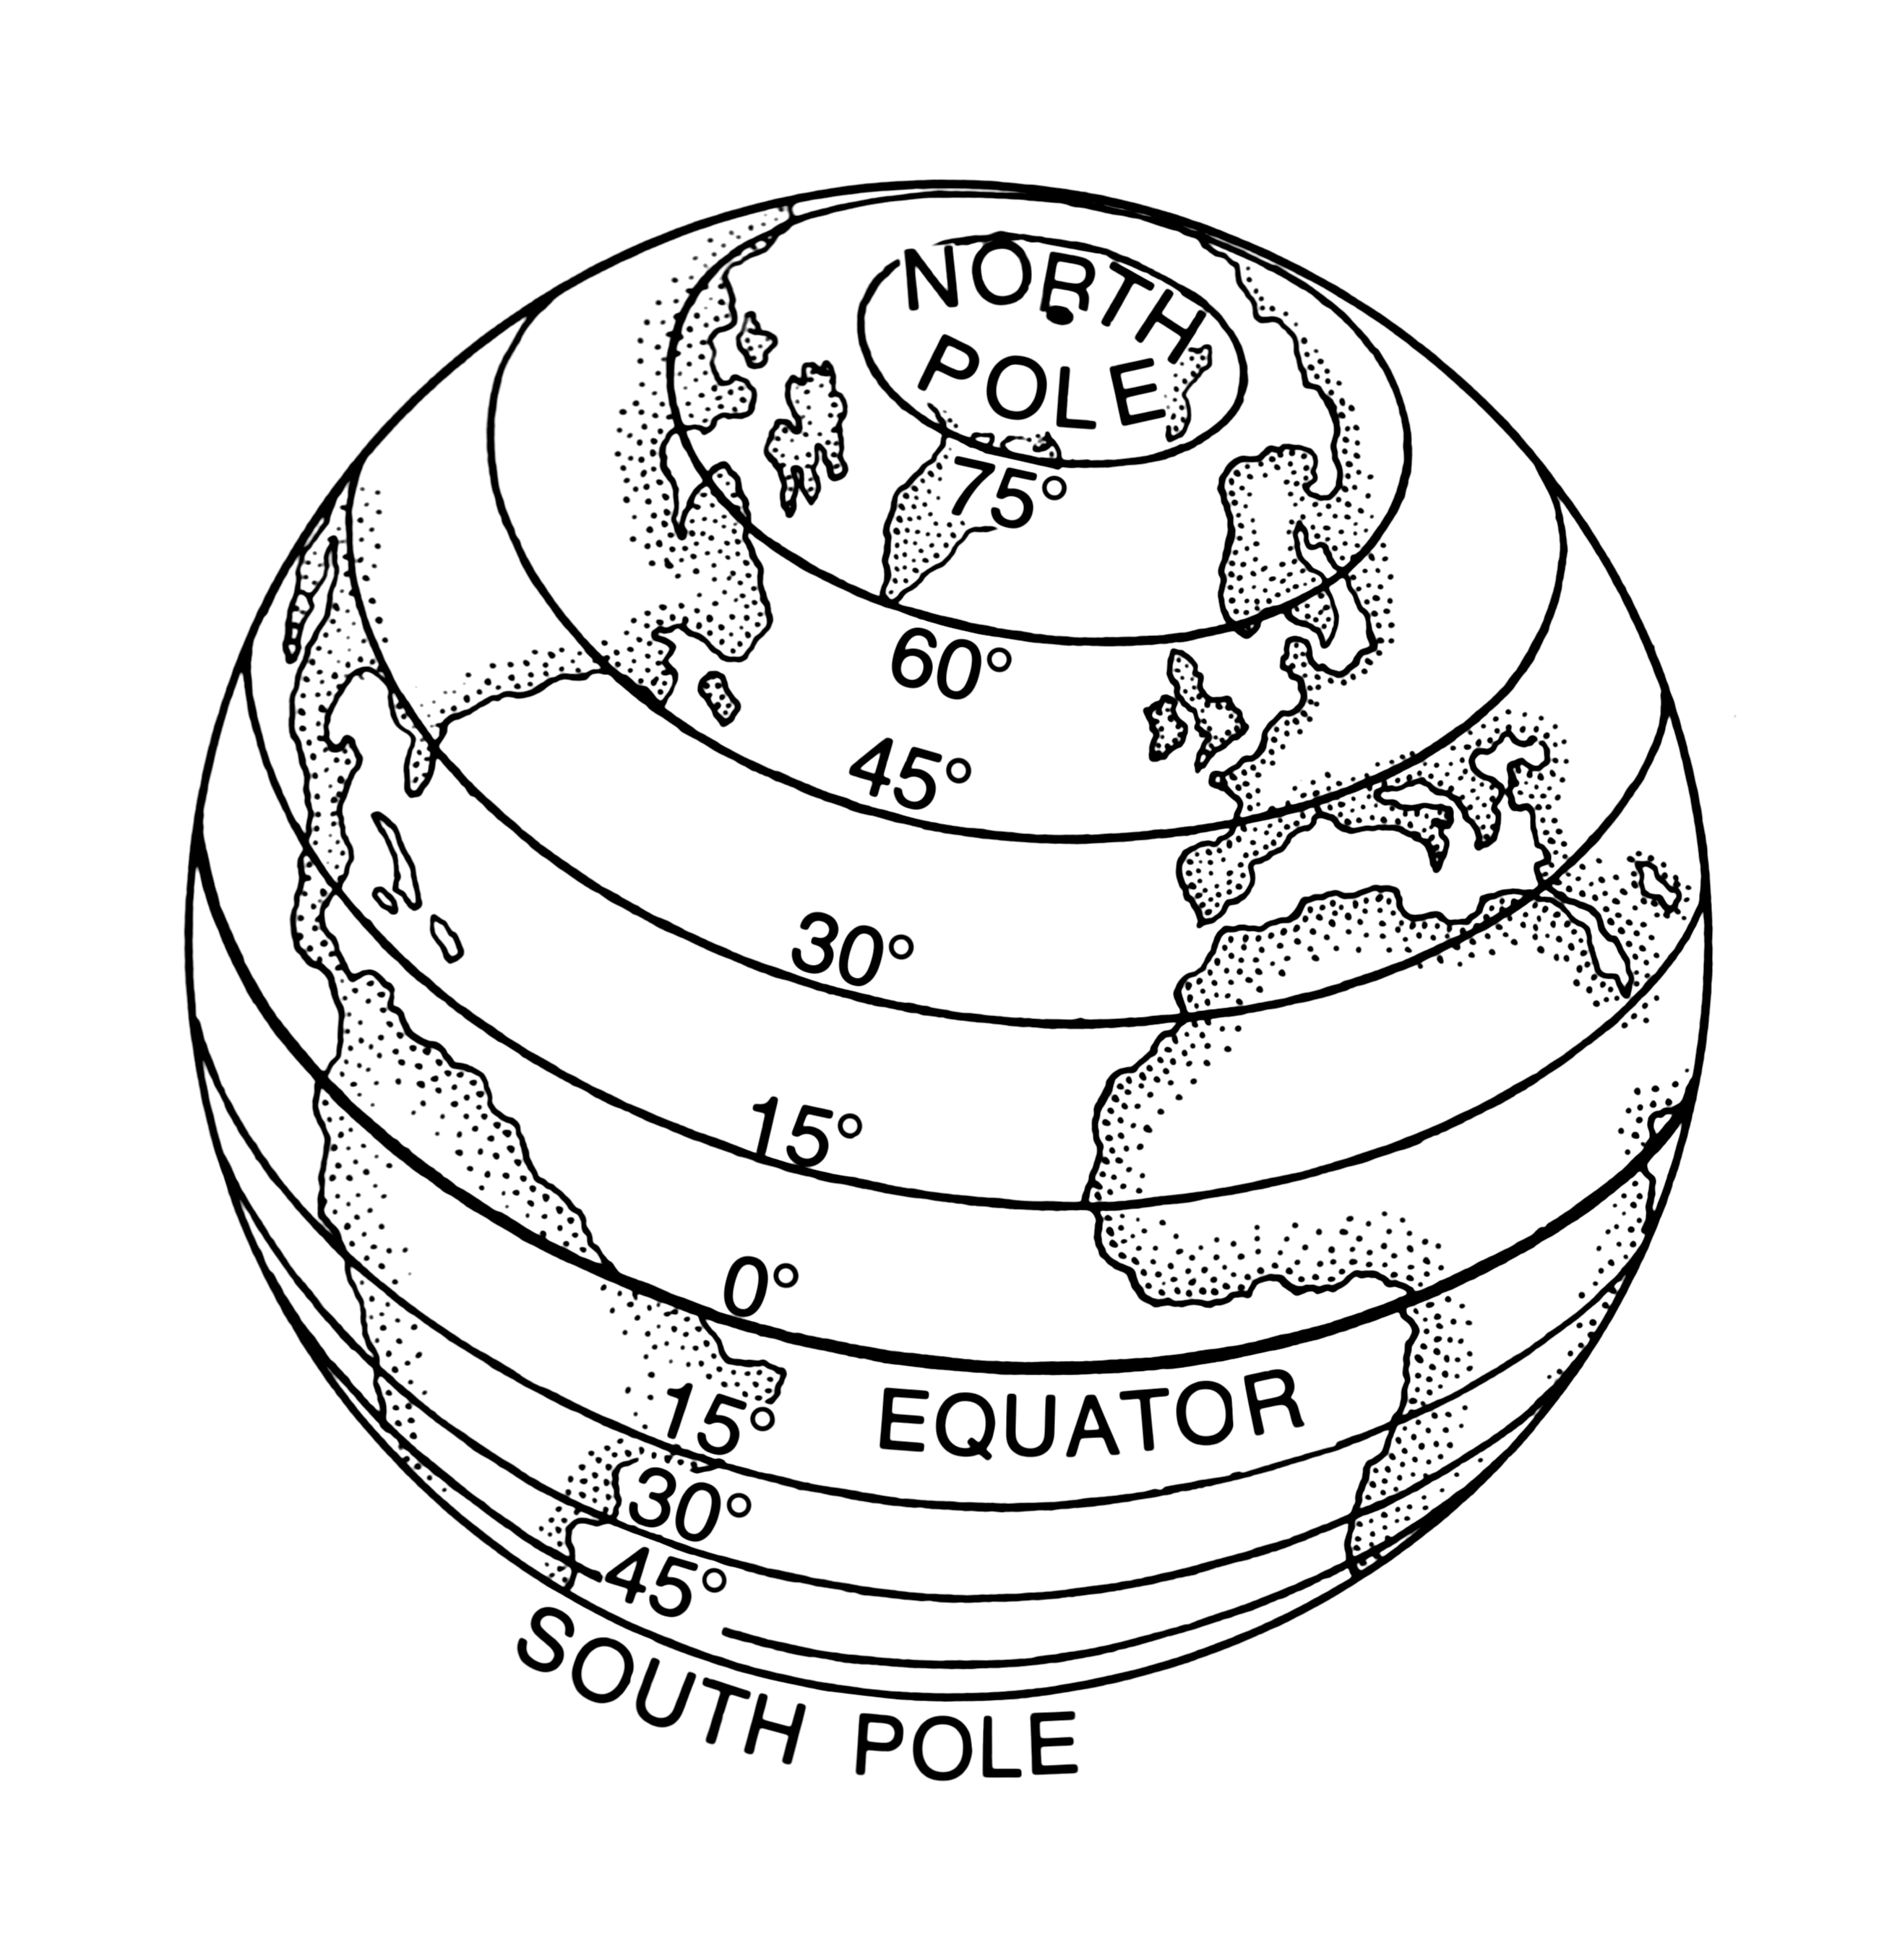
\includegraphics[width=2in]{./RadianMeasureGraphics/Latitude_(PSF).png}

\end{center}

\smallskip

{\bf Solution.}  To use the formula $v = r \omega$, we first need to compute the angular velocity $\omega$.  The earth makes one revolution in 24 hours, and one revolution is $2 \pi$ radians, so $\omega = \frac{2 \pi \, \text{radians}}{24 \, \text{hours}} = \frac{\pi}{12 \, \text{hours}}$. Note that once again, we are identifying angles in radian measure as real numbers so we can drop the `radian' units as they are dimensionless.  Also note that  for simplicity's sake, we assume that we are viewing the rotation of the earth as counter-clockwise so $\omega > 0$.  Hence, the linear velocity is \[ v = 2960 \, \text{miles} \cdot \frac{\pi}{12 \, \text{hours}} \approx 775 \, \frac{\text{miles}}{\text{hour}}\]  \qed

\end{ex}

It is worth noting that the quantity $\frac{1 \, \text{revolution}}{24 \, \text{hours}}$ in Example \ref{EarthRotationEx} is called the \index{frequency ! ordinary} \index{ordinary frequency} \textbf{ordinary frequency} of the motion and is usually denoted by the variable $f$.  The ordinary frequency is a measure of how often an object makes a complete cycle of the motion.  The fact that $\omega = 2\pi f$ suggests that $\omega$ is also a frequency.  Indeed, it is called the \index{frequency ! angular} \index{angular frequency} \textbf{angular frequency} of the motion.  On a related note, the quantity $T = \frac{1}{f}$ is called the \index{period ! circular motion}\textbf{period} of the motion and is the amount of time it takes for the object to complete one cycle of the motion.  In the scenario of Example \ref{EarthRotationEx}, the period of the motion is 24 hours, or one day.  

\smallskip

The concepts of frequency and period help frame the equation $v = r \omega$ in a new light.  That is, if $\omega$ is fixed, points which are farther from the center of rotation need to travel faster to maintain the same angular frequency since they have farther to travel to make one revolution in one period's time.  The distance of the object to the center of rotation is the radius of the circle, $r$, and is the `magnification factor' which relates $\omega$ and $v$. We will have more to say about frequencies and periods in Section \ref{GraphsofSineandCosine}.  While we have exhaustively discussed velocities associated with circular motion, we have yet to discuss a more natural question: if an object is moving on a circular path of radius $r$ with a fixed angular velocity (frequency) $\omega$, what is the position of the object at time $t$?  The answer to this question is the very heart of Trigonometry and is answered in the next section.   

\newpage

\subsection{Exercises}

\documentclass{ximera}

\begin{document}
	\author{Stitz-Zeager}
	\xmtitle{TITLE}





In Exercises \ref{orientedanglefirst} - \ref{orientedanglelast}, graph the oriented angle in standard position. Classify each angle according to where its terminal side lies and then give two coterminal angles, one of which is positive and the other negative.


\begin{multicols}{4} 

\begin{enumerate}


\item $\dfrac{\pi}{3}$
\item $\dfrac{5\pi}{6}$
\item $-\dfrac{11\pi}{3}$
\item $\dfrac{5\pi}{4}$

\setcounter{HW}{\value{enumi}}

\end{enumerate}

\end{multicols}

\begin{multicols}{4} 

\begin{enumerate}

\setcounter{enumi}{\value{HW}}

\item $\dfrac{3\pi}{4}$
\item $-\dfrac{\pi}{3}$ \vphantom{$\dfrac{11\pi}{6}$}
\item $\dfrac{7\pi}{2}$
\item $\dfrac{\pi}{4}$ \vphantom{$\dfrac{11\pi}{6}$}

\setcounter{HW}{\value{enumi}}

\end{enumerate}

\end{multicols}

\begin{multicols}{4} 

\begin{enumerate}

\setcounter{enumi}{\value{HW}}

\item $-\dfrac{\pi}{2}$ \vphantom{$\dfrac{11\pi}{6}$}
\item $\dfrac{7\pi}{6}$
\item $-\dfrac{5\pi}{3}$
\item $3\pi$ \vphantom{$\dfrac{11\pi}{6}$}

\setcounter{HW}{\value{enumi}}

\end{enumerate}

\end{multicols}

\begin{multicols}{4} 

\begin{enumerate}

\setcounter{enumi}{\value{HW}}

\item  $-2\pi$ \vphantom{$\dfrac{11\pi}{6}$}
\item $-\dfrac{\pi}{4}$ \vphantom{$\dfrac{11\pi}{6}$}
\item $\dfrac{15\pi}{4}$
\item $-\dfrac{13\pi}{6}$ \label{orientedanglelast}

\setcounter{HW}{\value{enumi}}

\end{enumerate}

\end{multicols}

In Exercises \ref{degreetoradianfirst} - \ref{degreetoradianlast}, convert the angle from degree measure into radian measure, giving the exact value in terms of $\pi$.

\begin{multicols}{4} 

\begin{enumerate}

\setcounter{enumi}{\value{HW}}

\item $0^{\circ}$ \label{degreetoradianfirst}
\item $240^{\circ}$
\item $135^{\circ}$
\item $-270^{\circ}$

\setcounter{HW}{\value{enumi}}

\end{enumerate}

\end{multicols}

\begin{multicols}{4} 

\begin{enumerate}

\setcounter{enumi}{\value{HW}}

\item $-315^{\circ}$
\item $150^{\circ}$
\item $45^{\circ}$
\item $-225^{\circ}$ \label{degreetoradianlast}

\setcounter{HW}{\value{enumi}}

\end{enumerate}

\end{multicols}

In Exercises \ref{radiantodegreefirst} - \ref{radiantodegreelast}, convert the angle from radian measure into degree measure.

\begin{multicols}{4} 

\begin{enumerate}

\setcounter{enumi}{\value{HW}}

\item $\pi$ \vphantom{$\dfrac{11\pi}{6}$} \label{radiantodegreefirst}
\item $-\dfrac{2\pi}{3}$
\item $\dfrac{7\pi}{6}$
\item $\dfrac{11\pi}{6}$

\setcounter{HW}{\value{enumi}}

\end{enumerate}

\end{multicols}

\begin{multicols}{4} 

\begin{enumerate}

\setcounter{enumi}{\value{HW}}

\item $\dfrac{\pi}{3}$ \vphantom{$\dfrac{11\pi}{6}$}
\item $\dfrac{5\pi}{3}$
\item $-\dfrac{\pi}{6}$ \vphantom{$\dfrac{11\pi}{6}$}
\item $\dfrac{\pi}{2}$ \vphantom{$\dfrac{11\pi}{6}$} \label{radiantodegreelast}

\setcounter{HW}{\value{enumi}}

\end{enumerate}

\end{multicols}


In Exercises \ref{orientedarcfirst} - \ref{orientedarclast}, sketch the oriented arc on the Unit Circle which  corresponds to the given real number. 

\begin{multicols}{5} 

\begin{enumerate}

\setcounter{enumi}{\value{HW}}

\item $t=\frac{5 \pi}{6}$ \label{orientedarcfirst}

\item $t=-\pi$

\item $t = 6$

\item  $t = -2$

\item  $t = 12$ \label{orientedarclast}

\setcounter{HW}{\value{enumi}}

\end{enumerate}

\end{multicols}

\begin{enumerate}

\setcounter{enumi}{\value{HW}}

\item  \label{spinningyoyo} A yo-yo which is 2.25 inches in diameter spins at a rate of 4500 revolutions per minute.  How fast is the edge of the yo-yo spinning in miles per hour?  Round your answer to two decimal places.

\item  How many revolutions per minute would the yo-yo in exercise \ref{spinningyoyo} have to complete if the edge of the yo-yo is to be spinning at a rate of 42 miles per hour?  Round your answer to two decimal places.

\item  \label{yoyotrick} In the yo-yo trick `Around the World,' the performer throws the yo-yo so it sweeps out a vertical circle whose radius is the yo-yo string. If the yo-yo string is 28 inches long and the yo-yo takes 3 seconds to complete one revolution of the circle, compute the speed of the yo-yo in miles per hour.  Round your answer to two decimal places.

\item A computer hard drive contains a circular disk with diameter 2.5 inches and spins at a rate of 7200 revolutions per minute.  Find the linear speed of a point on the edge of the disk in miles per hour. \label{harddrive} 

\item A rock got stuck in the tread of my tire and when I was driving 70 miles per hour, the rock came loose and hit the inside of the wheel well of the car.  How fast, in miles per hour, was the rock traveling when it came out of the tread?  (The tire has a diameter of 23 inches.)

\item The Giant Wheel at Cedar Point is a circle with diameter 128 feet which sits on an 8 foot tall platform making its overall height is 136 feet.  (Remember this from Exercise \ref{giantwheelcircle} in Section \ref{Circles}?)  It completes two revolutions in 2 minutes and 7 seconds.\footnote{Source: \href{http://www.cedarpoint.com/public/park/rides/tranquil/giant_wheel.cfm}{\underline{Cedar Point's webpage}}.}  Assuming the riders are at the edge of the circle, how fast are they traveling in miles per hour?
\label{giantwheelmotion}

\item  Consider the circle of radius $r$ pictured below with central angle $\theta$, measured in radians,  and subtended arc of length $s$.  Prove that the area of the shaded sector is $A = \frac{1}{2} r^{2} \theta$. 

(Hint: Use the proportion  $\frac{A}{\text{area of the circle}} = \frac{s}{\text{circumference of the circle}}$.)
\label{circularsectorarea}

\begin{center}

\begin{mfpic}[20]{-5}{5}{-5}{5}
 \drawcolor[gray]{0.7}
\circle{(0,0),3}
\fillcolor[gray]{0.7}
\gfill \plrregion{0,60,5}{3}
\drawcolor{black}
\polyline{(3, 0), (0,0), (1.5, 2.598)}
\arrow \reverse \arrow \parafcn{5, 55, 5}{1.5*dir(t)}
\point[4pt]{(0,0)}
\tlabel[cc](1.732, 1){$\theta$}
\penwd{1.5pt}
\parafcn{0,60,5}{3*dir(t)}
\tlabel[cc](3.0311,1.75){$s$}
\tlabel[cc](1.5,-0.5){$r$}
\tlabel[cc](0.5,1.5){$r$}
\end{mfpic}

\end{center}

\setcounter{HW}{\value{enumi}}

\end{enumerate}

In Exercises \ref{sectorfirst} - \ref{sectorlast}, use the result of Exercise \ref{circularsectorarea} to compute the areas of the circular sectors with the given central angles and radii.

\begin{multicols}{3} 

\begin{enumerate}

\setcounter{enumi}{\value{HW}}

\item $\theta = \dfrac{\pi}{6}, \; r = 12$ \vphantom{$\dfrac{5\pi}{4}$} \label{sectorfirst}
\item $\theta = \dfrac{5\pi}{4}, \; r = 100$
\item $\theta = 330^{\circ}, \; r = 9.3$ \vphantom{$\dfrac{5\pi}{4}$}

\setcounter{HW}{\value{enumi}}

\end{enumerate}

\end{multicols}

\begin{multicols}{3} 

\begin{enumerate}

\setcounter{enumi}{\value{HW}}

\item $\theta =\pi, \; r = 1$
\item $\theta = 240^{\circ}, \; r = 5$
\item $\theta = 1^{\circ}, \; r = 117$ \label{sectorlast}

\setcounter{HW}{\value{enumi}}

\end{enumerate}

\end{multicols}

\begin{enumerate}

\setcounter{enumi}{\value{HW}}

\item Imagine a rope tied around the Earth at the equator.  Show that you need to add only $2\pi$ feet of length to the rope in order to lift it one foot above the ground around the entire equator.  (You do NOT need to know the radius of the Earth to show this.)

\item With the help of your classmates, look for a proof that $\pi$ is indeed a constant.

\end{enumerate}

\newpage

\subsection{Answers}


\begin{multicols}{2} \raggedcolumns

\begin{enumerate}


\item $\dfrac{\pi}{3}$  is a Quadrant I angle\\
coterminal with $\dfrac{7\pi}{3}$ and $-\dfrac{5\pi}{3}$ 

\begin{mfpic}[12]{-5}{5}{-5}{5}
\drawcolor[gray]{0.7}
\axes
\xmarks{-4,-3,-2,-1,1,2,3,4}
\ymarks{-4,-3,-2,-1,1,2,3,4}
\tlabel(5,-0.5){\scriptsize $x$}
\tlabel(0.25,4.75){\scriptsize $y$}
\drawcolor{black}
\arrow \arc[c]{(0,0), (2.5,-0.1), 55}
\penwd{1.25pt}
\arrow \reverse \arrow \polyline{(2.5, 4.3301), (0,0), (5,0)}
\point[4pt]{(0,0)}
\tlpointsep{5pt}
\scriptsize
\axislabels {x}{{$-4 \hspace{7pt}$} -4, {$-3 \hspace{7pt}$} -3, {$-2 \hspace{7pt}$} -2, {$-1 \hspace{7pt}$} -1, {$1$} 1, {$2$} 2, {$3$} 3, {$4$} 4}
\axislabels {y}{{$-1$} -1, {$-2$} -2, {$-3$} -3, {$-4$} -4, {$1$} 1, {$2$} 2, {$3$} 3, {$4$} 4}
\normalsize
\end{mfpic}

\item $\dfrac{5\pi}{6}$ is a Quadrant II angle\\
coterminal with $\dfrac{17\pi}{6}$ and $-\dfrac{7\pi}{6}$

\begin{mfpic}[12]{-5}{5}{-5}{5}
\drawcolor[gray]{0.7}
\axes
\xmarks{-4,-3,-2,-1,1,2,3,4}
\ymarks{-4,-3,-2,-1,1,2,3,4}
\tlabel(5,-0.5){\scriptsize $x$}
\tlabel(0.25,4.75){\scriptsize $y$}
\drawcolor{black}
\arrow \arc[c]{(0,0), (2.5,0.1), 145}
\penwd{1.25pt}
\arrow \reverse \arrow \polyline{(-4.3301, 2.5), (0,0), (5,0)}
\point[4pt]{(0,0)}
\tlpointsep{5pt}
\scriptsize
\axislabels {x}{{$-4 \hspace{7pt}$} -4, {$-3 \hspace{7pt}$} -3, {$-2 \hspace{7pt}$} -2, {$-1 \hspace{7pt}$} -1, {$1$} 1, {$2$} 2, {$3$} 3, {$4$} 4}
\axislabels {y}{{$-1$} -1, {$-2$} -2, {$-3$} -3, {$-4$} -4, {$1$} 1, {$2$} 2, {$3$} 3, {$4$} 4}
\normalsize
\end{mfpic}

\setcounter{HW}{\value{enumi}}

\end{enumerate}

\end{multicols}

\begin{multicols}{2} \raggedcolumns

\begin{enumerate}

\setcounter{enumi}{\value{HW}}

\item $-\dfrac{11\pi}{3}$ \vphantom{$\dfrac{17\pi}{6}$} is a Quadrant I angle\\
coterminal with $\dfrac{\pi}{3}$ and $-\dfrac{5\pi}{3}$ \vphantom{$\dfrac{17\pi}{4}$}

\begin{mfpic}[12]{-5}{5}{-5}{5}
\drawcolor[gray]{0.7}
\axes
\xmarks{-4,-3,-2,-1,1,2,3,4}
\ymarks{-4,-3,-2,-1,1,2,3,4}
\tlabel(5,-0.5){\scriptsize $x$}
\tlabel(0.25,4.75){\scriptsize $y$}
\drawcolor{black}
\arrow \parafcn{0,655,5}{(t+100)*dir(0-t)/400}
\penwd{1.25pt}
\arrow \reverse \arrow \polyline{(2.5, 4.3301), (0,0), (5,0)}
\point[4pt]{(0,0)}
\tlpointsep{5pt}
\scriptsize
\axislabels {x}{{$-4 \hspace{7pt}$} -4, {$-3 \hspace{7pt}$} -3, {$-2 \hspace{7pt}$} -2, {$-1 \hspace{7pt}$} -1, {$1$} 1, {$2$} 2, {$3$} 3, {$4$} 4}
\axislabels {y}{{$-1$} -1, {$-2$} -2, {$-3$} -3, {$-4$} -4, {$1$} 1, {$2$} 2, {$3$} 3, {$4$} 4}
\normalsize
\end{mfpic} 

\item $\dfrac{5\pi}{4}$ is a Quadrant III angle\\
coterminal with $\dfrac{13\pi}{4}$ and $-\dfrac{3\pi}{4}$

\begin{mfpic}[12]{-5}{5}{-5}{5}
\drawcolor[gray]{0.7}
\axes
\xmarks{-4,-3,-2,-1,1,2,3,4}
\ymarks{-4,-3,-2,-1,1,2,3,4}
\tlabel(5,-0.5){\scriptsize $x$}
\tlabel(0.25,4.75){\scriptsize $y$}
\drawcolor{black}
\arrow \arc[c]{(0,0), (2.5,0.1), 220}
\penwd{1.25pt}
\arrow \reverse \arrow \polyline{(-3.5355, -3.5355), (0,0), (5,0)}
\point[4pt]{(0,0)}
\tlpointsep{5pt}
\scriptsize
\axislabels {x}{{$-4 \hspace{7pt}$} -4, {$-3 \hspace{7pt}$} -3, {$-2 \hspace{7pt}$} -2, {$-1 \hspace{7pt}$} -1, {$1$} 1, {$2$} 2, {$3$} 3, {$4$} 4}
\axislabels {y}{{$-1$} -1, {$-2$} -2, {$-3$} -3, {$-4$} -4, {$1$} 1, {$2$} 2, {$3$} 3, {$4$} 4}
\normalsize
\end{mfpic}

\setcounter{HW}{\value{enumi}}

\end{enumerate}

\end{multicols}

\begin{multicols}{2} \raggedcolumns

\begin{enumerate}

\setcounter{enumi}{\value{HW}}

\item $\dfrac{3\pi}{4}$ is a Quadrant II angle\\
coterminal with $\dfrac{11\pi}{4}$ and $-\dfrac{5\pi}{4}$

\begin{mfpic}[12]{-5}{5}{-5}{5}
\drawcolor[gray]{0.7}
\axes
\xmarks{-4,-3,-2,-1,1,2,3,4}
\ymarks{-4,-3,-2,-1,1,2,3,4}
\tlabel(5,-0.5){\scriptsize $x$}
\tlabel(0.25,4.75){\scriptsize $y$}
\drawcolor{black}
\arrow \arc[c]{(0,0), (2.5,0.1), 130}
\penwd{1.25pt}
\arrow \reverse \arrow \polyline{(-3.5355, 3.5355), (0,0), (5,0)}
\point[4pt]{(0,0)}
\tlpointsep{5pt}
\scriptsize
\axislabels {x}{{$-4 \hspace{7pt}$} -4, {$-3 \hspace{7pt}$} -3, {$-2 \hspace{7pt}$} -2, {$-1 \hspace{7pt}$} -1, {$1$} 1, {$2$} 2, {$3$} 3, {$4$} 4}
\axislabels {y}{{$-1$} -1, {$-2$} -2, {$-3$} -3, {$-4$} -4, {$1$} 1, {$2$} 2, {$3$} 3, {$4$} 4}
\normalsize
\end{mfpic}

\item $-\dfrac{\pi}{3}$ \vphantom{$\dfrac{17\pi}{4}$} is a Quadrant IV angle\\
coterminal with $\dfrac{5\pi}{3}$ and $-\dfrac{7\pi}{3}$ \vphantom{$\dfrac{17\pi}{4}$}

\begin{mfpic}[12]{-5}{5}{-5}{5}
\drawcolor[gray]{0.7}
\axes
\xmarks{-4,-3,-2,-1,1,2,3,4}
\ymarks{-4,-3,-2,-1,1,2,3,4}
\tlabel(5,-0.5){\scriptsize $x$}
\tlabel(0.25,4.75){\scriptsize $y$}
\drawcolor{black}
\arrow \arc[c]{(0,0), (2.5,-0.1), -55}
\penwd{1.25pt}
\arrow \reverse \arrow \polyline{(2.5, -4.3301), (0,0), (5,0)}
\point[4pt]{(0,0)}
\tlpointsep{5pt}
\scriptsize
\axislabels {x}{{$-4 \hspace{7pt}$} -4, {$-3 \hspace{7pt}$} -3, {$-2 \hspace{7pt}$} -2, {$-1 \hspace{7pt}$} -1, {$1$} 1, {$2$} 2, {$3$} 3, {$4$} 4}
\axislabels {y}{{$-1$} -1, {$-2$} -2, {$-3$} -3, {$-4$} -4, {$1$} 1, {$2$} 2, {$3$} 3, {$4$} 4}
\normalsize
\end{mfpic}

\setcounter{HW}{\value{enumi}}

\end{enumerate}

\end{multicols}

\begin{multicols}{2} \raggedcolumns

\begin{enumerate}

\setcounter{enumi}{\value{HW}}

\item $\dfrac{7\pi}{2}$ lies on the negative $y$-axis \vphantom{$\dfrac{17\pi}{4}$}\\
coterminal with $\dfrac{3\pi}{2}$ and $-\dfrac{\pi}{2}$ \vphantom{$\dfrac{17\pi}{4}$}

\begin{mfpic}[12]{-5}{5}{-5}{5}
\drawcolor[gray]{0.7}
\axes
\xmarks{-4,-3,-2,-1,1,2,3,4}
\ymarks{-4,-3,-2,-1,1,2,3,4}
\tlabel(5,-0.5){\scriptsize $x$}
\tlabel(0.25,4.75){\scriptsize $y$}
\drawcolor{black}
\arrow \parafcn{0,625,5}{(t+100)*dir(t)/400}
\penwd{1.25pt}
\arrow \reverse \arrow \polyline{(0, -5), (0,0), (5,0)}
\point[4pt]{(0,0)}
\tlpointsep{5pt}
\scriptsize
\axislabels {x}{{$-4 \hspace{7pt}$} -4, {$-3 \hspace{7pt}$} -3, {$-2 \hspace{7pt}$} -2, {$-1 \hspace{7pt}$} -1, {$1$} 1, {$2$} 2, {$3$} 3, {$4$} 4}
\axislabels {y}{{$-1$} -1, {$-2$} -2, {$-3$} -3, {$-4$} -4, {$1$} 1, {$2$} 2, {$3$} 3, {$4$} 4}
\normalsize
\end{mfpic} 

\item $\dfrac{\pi}{4}$ is a Quadrant I angle \vphantom{$\dfrac{17\pi}{2}$}\\
coterminal with $\dfrac{9 \pi}{4}$ and $-\dfrac{7\pi}{4}$

\begin{mfpic}[12]{-5}{5}{-5}{5}
\drawcolor[gray]{0.7}
\axes
\xmarks{-4,-3,-2,-1,1,2,3,4}
\ymarks{-4,-3,-2,-1,1,2,3,4}
\tlabel(5,-0.5){\scriptsize $x$}
\tlabel(0.25,4.75){\scriptsize $y$}
\drawcolor{black}
\arrow \arc[c]{(0,0), (2.5, 0.1), 40}
\penwd{1.25pt}
\arrow \reverse \arrow \polyline{(3.5355, 3.5355), (0,0), (5,0)}
\point[4pt]{(0,0)}
\tlpointsep{5pt}
\scriptsize
\axislabels {x}{{$-4 \hspace{7pt}$} -4, {$-3 \hspace{7pt}$} -3, {$-2 \hspace{7pt}$} -2, {$-1 \hspace{7pt}$} -1, {$1$} 1, {$2$} 2, {$3$} 3, {$4$} 4}
\axislabels {y}{{$-1$} -1, {$-2$} -2, {$-3$} -3, {$-4$} -4, {$1$} 1, {$2$} 2, {$3$} 3, {$4$} 4}
\normalsize
\end{mfpic}

\setcounter{HW}{\value{enumi}}

\end{enumerate}

\end{multicols}

\begin{multicols}{2} \raggedcolumns

\begin{enumerate}

\setcounter{enumi}{\value{HW}}

\item $-\dfrac{\pi}{2}$ lies on the negative $y$-axis \vphantom{$\dfrac{17\pi}{4}$}\\
coterminal with $\dfrac{3\pi}{2}$ and $-\dfrac{5\pi}{2}$

\begin{mfpic}[12]{-5}{5}{-5}{5}
\drawcolor[gray]{0.7}
\axes
\xmarks{-4,-3,-2,-1,1,2,3,4}
\ymarks{-4,-3,-2,-1,1,2,3,4}
\tlabel(5,-0.5){\scriptsize $x$}
\tlabel(0.25,4.75){\scriptsize $y$}
\drawcolor{black}
\arrow \arc[c]{(0,0), (2.5, -0.1), -85}
\penwd{1.25pt}
 \arrow \reverse \arrow \polyline{(0, -5), (0,0), (5,0)}
\point[4pt]{(0,0)}
\tlpointsep{5pt}
\scriptsize
\axislabels {x}{{$-4 \hspace{7pt}$} -4, {$-3 \hspace{7pt}$} -3, {$-2 \hspace{7pt}$} -2, {$-1 \hspace{7pt}$} -1, {$1$} 1, {$2$} 2, {$3$} 3, {$4$} 4}
\axislabels {y}{{$-1$} -1, {$-2$} -2, {$-3$} -3, {$-4$} -4, {$1$} 1, {$2$} 2, {$3$} 3, {$4$} 4}
\normalsize
\end{mfpic}

\item $\dfrac{7\pi}{6}$ is a Quadrant III angle\\
coterminal with $\dfrac{19 \pi}{6}$ and $-\dfrac{5\pi}{6}$

\begin{mfpic}[12]{-5}{5}{-5}{5}
\drawcolor[gray]{0.7}
\axes
\xmarks{-4,-3,-2,-1,1,2,3,4}
\ymarks{-4,-3,-2,-1,1,2,3,4}
\tlabel(5,-0.5){\scriptsize $x$}
\tlabel(0.25,4.75){\scriptsize $y$}
\drawcolor{black}
\arrow \arc[c]{(0,0), (2.5, 0.1), 205}
\penwd{1.25pt}
\arrow \reverse \arrow \polyline{(-4.3301,-2.5), (0,0), (5,0)}
\point[4pt]{(0,0)}
\tlpointsep{5pt}
\scriptsize
\axislabels {x}{{$-4 \hspace{7pt}$} -4, {$-3 \hspace{7pt}$} -3, {$-2 \hspace{7pt}$} -2, {$-1 \hspace{7pt}$} -1, {$1$} 1, {$2$} 2, {$3$} 3, {$4$} 4}
\axislabels {y}{{$-1$} -1, {$-2$} -2, {$-3$} -3, {$-4$} -4, {$1$} 1, {$2$} 2, {$3$} 3, {$4$} 4}
\normalsize
\end{mfpic}

\setcounter{HW}{\value{enumi}}

\end{enumerate}

\end{multicols}

\begin{multicols}{2} \raggedcolumns

\begin{enumerate}

\setcounter{enumi}{\value{HW}}

\item $-\dfrac{5\pi}{3}$ is a Quadrant I angle \vphantom{$\dfrac{17\pi}{4}$} \\
coterminal with $\dfrac{\pi}{3}$ and $-\dfrac{11\pi}{3}$ \vphantom{$\dfrac{17\pi}{4}$}

\begin{mfpic}[12]{-5}{5}{-5}{5}
\drawcolor[gray]{0.7}
\axes
\xmarks{-4,-3,-2,-1,1,2,3,4}
\ymarks{-4,-3,-2,-1,1,2,3,4}
\tlabel(5,-0.5){\scriptsize $x$}
\tlabel(0.25,4.75){\scriptsize $y$}
\drawcolor{black}
\arrow \arc[c]{(0,0), (2.5, -0.1), -295}
\penwd{1.25pt}
\arrow \reverse \arrow \polyline{(2.5, 4.3301), (0,0), (5,0)}
\point[4pt]{(0,0)}
\tlpointsep{5pt}
\scriptsize
\axislabels {x}{{$-4 \hspace{7pt}$} -4, {$-3 \hspace{7pt}$} -3, {$-2 \hspace{7pt}$} -2, {$-1 \hspace{7pt}$} -1, {$1$} 1, {$2$} 2, {$3$} 3, {$4$} 4}
\axislabels {y}{{$-1$} -1, {$-2$} -2, {$-3$} -3, {$-4$} -4, {$1$} 1, {$2$} 2, {$3$} 3, {$4$} 4}
\normalsize
\end{mfpic}

\item $3\pi$ lies on the negative $x$-axis \vphantom{$\dfrac{17\pi}{4}$} \\
coterminal with $\pi$ and $-\pi$ \vphantom{$\dfrac{17\pi}{4}$}

\begin{mfpic}[12]{-5}{5}{-5}{5}
\drawcolor[gray]{0.7}
\axes
\xmarks{-4,-3,-2,-1,1,2,3,4}
\ymarks{-4,-3,-2,-1,1,2,3,4}
\tlabel(5,-0.5){\scriptsize $x$}
\tlabel(0.25,4.75){\scriptsize $y$}
\drawcolor{black}
\arrow \parafcn{0,535,5}{(t+100)*dir(t)/400}
\penwd{1.25pt}
\arrow \reverse \arrow \polyline{(-5,0), (0,0), (5,0)}
\point[4pt]{(0,0)}
\tlpointsep{5pt}
\scriptsize
\axislabels {x}{{$-4 \hspace{7pt}$} -4, {$-3 \hspace{7pt}$} -3, {$-2 \hspace{7pt}$} -2, {$-1 \hspace{7pt}$} -1, {$1$} 1, {$2$} 2, {$3$} 3, {$4$} 4}
\axislabels {y}{{$-1$} -1, {$-2$} -2, {$-3$} -3, {$-4$} -4, {$1$} 1, {$2$} 2, {$3$} 3, {$4$} 4}
\normalsize
\end{mfpic} 

\setcounter{HW}{\value{enumi}}

\end{enumerate}

\end{multicols}

\begin{multicols}{2} \raggedcolumns

\begin{enumerate}

\setcounter{enumi}{\value{HW}}

\item $-2\pi$ lies on the positive $x$-axis \vphantom{$\dfrac{17\pi}{4}$} \\
coterminal with $2\pi$ and $-4\pi$ \vphantom{$\dfrac{17\pi}{4}$}

\begin{mfpic}[12]{-5}{5}{-5}{5}
\drawcolor[gray]{0.7}
\axes
\xmarks{-4,-3,-2,-1,1,2,3,4}
\ymarks{-4,-3,-2,-1,1,2,3,4}
\tlabel(5,-0.5){\scriptsize $x$}
\tlabel(0.25,4.75){\scriptsize $y$}
\drawcolor{black}
\arrow \parafcn{0,355,5}{(t+100)*dir(0-t)/300}
\penwd{1.25pt}
\point[4pt]{(0,0)}
\arrow \polyline{(0,0), (5,0)}
\tlpointsep{5pt}
\scriptsize
\axislabels {x}{{$-4 \hspace{7pt}$} -4, {$-3 \hspace{7pt}$} -3, {$-2 \hspace{7pt}$} -2, {$-1 \hspace{7pt}$} -1, {$1$} 1, {$2$} 2, {$3$} 3, {$4$} 4}
\axislabels {y}{{$-1$} -1, {$-2$} -2, {$-3$} -3, {$-4$} -4, {$1$} 1, {$2$} 2, {$3$} 3, {$4$} 4}
\normalsize
\end{mfpic}

\item $-\dfrac{\pi}{4}$ is a Quadrant IV angle \vphantom{$\dfrac{17\pi}{4}$} \\
coterminal with $\dfrac{7 \pi}{4}$ and $-\dfrac{9\pi}{4}$

\begin{mfpic}[12]{-5}{5}{-5}{5}
\drawcolor[gray]{0.7}
\axes
\xmarks{-4,-3,-2,-1,1,2,3,4}
\ymarks{-4,-3,-2,-1,1,2,3,4}
\tlabel(5,-0.5){\scriptsize $x$}
\tlabel(0.25,4.75){\scriptsize $y$}
\drawcolor{black}
\arrow \arc[c]{(0,0), (2.5, -0.1), -40}
\penwd{1.25pt}
\arrow \reverse \arrow \polyline{(3.5355,-3.5355), (0,0), (5,0)}
\point[4pt]{(0,0)}
\tlpointsep{5pt}
\scriptsize
\axislabels {x}{{$-4 \hspace{7pt}$} -4, {$-3 \hspace{7pt}$} -3, {$-2 \hspace{7pt}$} -2, {$-1 \hspace{7pt}$} -1, {$1$} 1, {$2$} 2, {$3$} 3, {$4$} 4}
\axislabels {y}{{$-1$} -1, {$-2$} -2, {$-3$} -3, {$-4$} -4, {$1$} 1, {$2$} 2, {$3$} 3, {$4$} 4}
\normalsize
\end{mfpic}

\setcounter{HW}{\value{enumi}}

\end{enumerate}

\end{multicols}

\begin{multicols}{2} \raggedcolumns

\begin{enumerate}

\setcounter{enumi}{\value{HW}}

\item $\dfrac{15\pi}{4}$ is a Quadrant IV angle\\
coterminal with $\dfrac{7\pi}{4}$ and $-\dfrac{\pi}{4}$

\begin{mfpic}[12]{-5}{5}{-5}{5}
\drawcolor[gray]{0.7}
\axes
\xmarks{-4,-3,-2,-1,1,2,3,4}
\ymarks{-4,-3,-2,-1,1,2,3,4}
\tlabel(5,-0.5){\scriptsize $x$}
\tlabel(0.25,4.75){\scriptsize $y$}
\drawcolor{black}
\arrow \parafcn{0,670,5}{(t+100)*dir(t)/400}
\penwd{1.25pt}
\arrow \reverse \arrow \polyline{(3.5355,-3.5355), (0,0), (5,0)}
\point[4pt]{(0,0)}
\tlpointsep{5pt}
\scriptsize
\axislabels {x}{{$-4 \hspace{7pt}$} -4, {$-3 \hspace{7pt}$} -3, {$-2 \hspace{7pt}$} -2, {$-1 \hspace{7pt}$} -1, {$1$} 1, {$2$} 2, {$3$} 3, {$4$} 4}
\axislabels {y}{{$-1$} -1, {$-2$} -2, {$-3$} -3, {$-4$} -4, {$1$} 1, {$2$} 2, {$3$} 3, {$4$} 4}
\normalsize
\end{mfpic} 

\item $-\dfrac{13\pi}{6}$ is a Quadrant IV angle\\
coterminal with $\dfrac{11\pi}{6}$ and $-\dfrac{\pi}{6}$

\begin{mfpic}[12]{-5}{5}{-5}{5}
\drawcolor[gray]{0.7}
\axes
\xmarks{-4,-3,-2,-1,1,2,3,4}
\ymarks{-4,-3,-2,-1,1,2,3,4}
\tlabel(5,-0.5){\scriptsize $x$}
\tlabel(0.25,4.75){\scriptsize $y$}
\drawcolor{black}
\arrow \parafcn{0,385,5}{(t+100)*dir(0-t)/300}
\penwd{1.25pt}
\arrow \reverse \arrow \polyline{(4.3301,-2.5), (0,0), (5,0)}
\point[4pt]{(0,0)}
\tlpointsep{5pt}
\scriptsize
\axislabels {x}{{$-4 \hspace{7pt}$} -4, {$-3 \hspace{7pt}$} -3, {$-2 \hspace{7pt}$} -2, {$-1 \hspace{7pt}$} -1, {$1$} 1, {$2$} 2, {$3$} 3, {$4$} 4}
\axislabels {y}{{$-1$} -1, {$-2$} -2, {$-3$} -3, {$-4$} -4, {$1$} 1, {$2$} 2, {$3$} 3, {$4$} 4}
\normalsize
\end{mfpic} 

\setcounter{HW}{\value{enumi}}

\end{enumerate}

\end{multicols}

\begin{multicols}{4}

\begin{enumerate}

\setcounter{enumi}{\value{HW}}

\item $0$ \vphantom{$\dfrac{17\pi}{4}$}
\item $\dfrac{4\pi}{3}$
\item $\dfrac{3\pi}{4}$
\item $-\dfrac{3\pi}{2}$

\setcounter{HW}{\value{enumi}}

\end{enumerate}

\end{multicols}

\begin{multicols}{4}

\begin{enumerate}

\setcounter{enumi}{\value{HW}}

\item $-\dfrac{7\pi}{4}$
\item $\dfrac{5\pi}{6}$
\item $\dfrac{\pi}{4}$ \vphantom{$\dfrac{17\pi}{4}$}
\item $-\dfrac{5\pi}{4}$

\setcounter{HW}{\value{enumi}}

\end{enumerate}

\end{multicols}

\begin{multicols}{4}

\begin{enumerate}

\setcounter{enumi}{\value{HW}}

\item $180^{\circ}$
\item $-120^{\circ}$
\item $210^{\circ}$
\item $330^{\circ}$

\setcounter{HW}{\value{enumi}}

\end{enumerate}

\end{multicols}

\begin{multicols}{4}

\begin{enumerate}

\setcounter{enumi}{\value{HW}}

\item $60^{\circ}$
\item $300^{\circ}$
\item $-30^{\circ}$
\item $90^{\circ}$

\setcounter{HW}{\value{enumi}}

\end{enumerate}

\end{multicols}

\newpage

\begin{multicols}{2} \raggedcolumns

\begin{enumerate}

\setcounter{enumi}{\value{HW}}

\item  $t = \dfrac{5\pi}{6}$

\begin{mfpic}[10]{-5}{5}{-5}{5}
\axes
\tlabel(5,-0.5){\scriptsize $x$}
\tlabel(0.5,5){\scriptsize $y$}
\tlabel(3.1,-0.75){\scriptsize $1$}
\tlabel(0.25,3.1){\scriptsize $1$}
\xmarks{-3 step 3 until 3}
\ymarks{-3 step 3 until 3}
\dotted \polyline{(0,0), (-4.3301,2.5)}
\drawcolor[gray]{0.7}
\circle{(0,0),3}
\drawcolor{black}
\penwd{1.5pt}
\arrow \parafcn{0, 150, 5}{3*dir(t)}
\end{mfpic} 

\item  $t = -\pi$ \vphantom{$\dfrac{5\pi}{6}$}

\begin{mfpic}[10]{-5}{5}{-5}{5}
\axes
\tlabel(5,-0.5){\scriptsize $x$}
\tlabel(0.5,5){\scriptsize $y$}
\tlabel(3.1,-0.75){\scriptsize $1$}
\tlabel(0.25,3.1){\scriptsize $1$}
\xmarks{-3 step 3 until 3}
\ymarks{-3 step 3 until 3}
\drawcolor[gray]{0.7}
\circle{(0,0),3}
\drawcolor{black}
\penwd{1.5pt}
\arrow \parafcn{0, 180, 5}{3*dir(-t)}
\end{mfpic} 

\setcounter{HW}{\value{enumi}}

\end{enumerate}

\end{multicols}

\begin{multicols}{2} \raggedcolumns

\begin{enumerate}

\setcounter{enumi}{\value{HW}}

\item  $t = 6$

\begin{mfpic}[10]{-5}{5}{-5}{5}
\axes
\tlabel(5,-0.5){\scriptsize $x$}
\tlabel(0.5,5){\scriptsize $y$}
\tlabel(3.1,-0.75){\scriptsize $1$}
\tlabel(0.25,3.1){\scriptsize $1$}
\xmarks{-3 step 3 until 3}
\ymarks{-3 step 3 until 3}
\dotted \polyline{(0,0), (4.801,-1.397)}
\drawcolor[gray]{0.7}
\circle{(0,0),3}
\drawcolor{black}
\penwd{1.5pt}
\arrow \parafcn{0, 343, 5}{3*dir(t)}
\end{mfpic} 

\item  $t = -2$

\begin{mfpic}[10]{-5}{5}{-5}{5}
\axes
\tlabel(4.5,-0.5){\scriptsize $x$}
\tlabel(0.5,4.5){\scriptsize $y$}
\tlabel(3.1,-0.75){\scriptsize $1$}
\tlabel(0.25,3.1){\scriptsize $1$}
\xmarks{-3 step 3 until 3}
\ymarks{-3 step 3 until 3}
\dotted \polyline{(0,0), (-2.081,-4.546)}
\drawcolor[gray]{0.7}
\circle{(0,0),3}
\drawcolor{black}
\penwd{1.5pt}
\arrow \parafcn{0, 114, 5}{3*dir(-t)}
\end{mfpic} 

\setcounter{HW}{\value{enumi}}

\end{enumerate}

\end{multicols}

%\begin{multicols}{2} 

\begin{enumerate}

\setcounter{enumi}{\value{HW}}

\item  $t = 12$  (between 1 and 2 revolutions)

\begin{mfpic}[10]{-5}{5}{-5}{5}
\axes
\tlabel(5,-0.5){\scriptsize $x$}
\tlabel(0.5,5){\scriptsize $y$}
\tlabel(3.1,-0.75){\scriptsize $1$}
\tlabel(0.25,3.1){\scriptsize $1$}
\xmarks{-3 step 3 until 3}
\ymarks{-3 step 3 until 3}
\dotted \polyline{(0,0), (4.219,-2.683)}
\drawcolor[gray]{0.7}
\circle{(0,0),3}
\drawcolor{black}
\penwd{1.5pt}
\arrow \parafcn{0, 687, 5}{3*dir(t)}
\end{mfpic} 

\setcounter{HW}{\value{enumi}}

\end{enumerate}

%\end{multicols}

\begin{multicols}{2}

\begin{enumerate}

\setcounter{enumi}{\value{HW}}

\item About 30.12 miles per hour
\item About 6274.52 revolutions per minute

\setcounter{HW}{\value{enumi}}

\end{enumerate}

\end{multicols}

\begin{multicols}{2}

\begin{enumerate}

\setcounter{enumi}{\value{HW}}

\item About 3.33 miles per hour
\item About 53.55 miles per hour

\setcounter{HW}{\value{enumi}}

\end{enumerate}

\end{multicols}

\begin{multicols}{2}

\begin{enumerate}

\setcounter{enumi}{\value{HW}}

\item 70 miles per hour
\item About 4.32 miles per hour

\setcounter{HW}{\value{enumi}}

\end{enumerate}

\end{multicols}

\begin{multicols}{2}

\begin{enumerate}

\setcounter{enumi}{\value{HW}}

\addtocounter{enumi}{1}

\item $12\pi$ square units
\item $6250\pi$ square units 

\setcounter{HW}{\value{enumi}}

\end{enumerate}

\end{multicols}

\begin{multicols}{2}

\begin{enumerate}

\setcounter{enumi}{\value{HW}}

\item $79.2825\pi \approx 249.07$ square units \vphantom{$\dfrac{\pi}{2}$}
\item $\dfrac{\pi}{2}$ square units

\setcounter{HW}{\value{enumi}}

\end{enumerate}

\end{multicols}

\enlargethispage{0.25in}

\vspace{-0.25in}

\begin{multicols}{2}

\begin{enumerate}

\setcounter{enumi}{\value{HW}}

\item $\dfrac{50\pi}{3}$ square units
\item $38.025 \pi \approx 119.46$ square units \vphantom{$\dfrac{50\pi}{3}$}

\end{enumerate}

\end{multicols}




\end{document}



\closegraphsfile

\end{document}
